\documentclass[border=2pt]{standalone}
\usepackage{tikz}
\usetikzlibrary{arrows.meta,positioning,calc,fit,backgrounds,shapes.geometric}
\usepackage{amsmath,amssymb}
\usepackage{times}
\definecolor{ink}{HTML}{243447}
\definecolor{cA}{HTML}{4477AA}
\definecolor{cB}{HTML}{CC6677}
\definecolor{cAu}{HTML}{44AA99}
\definecolor{cS}{HTML}{CCAA33}
\definecolor{grn}{HTML}{228833}
\definecolor{rose}{HTML}{AA3377}
\definecolor{inst}{HTML}{F2E3B3}
\tikzset{
 pap/.style={circle,draw=ink,line width=.6pt,minimum size=15pt,inner sep=0pt,font=\scriptsize\bfseries,text=white},
 aut/.style={rectangle,draw=ink,line width=.6pt,minimum size=13pt,inner sep=0pt,fill=cAu,font=\scriptsize\bfseries,text=white},
 sub/.style={diamond,draw=ink,line width=.6pt,minimum size=17pt,inner sep=0pt,fill=cS,font=\scriptsize\bfseries,text=white},
 gone/.style={draw=ink!35,fill=ink!8,text=ink!40,dashed},
 ed/.style={draw=ink,line width=.7pt},
 msg/.style={-{Stealth[length=4pt]},line width=.9pt,draw=rose},
 ptitle/.style={font=\footnotesize\bfseries,text=ink,anchor=west},
 note/.style={font=\scriptsize,text=ink,align=center},
}

\tikzset{
 stage/.style={draw=ink!50,rounded corners=3pt,line width=.5pt,minimum width=2.78cm,minimum height=2.5cm,anchor=north west},
 stnum/.style={circle,fill=ink,text=white,font=\scriptsize\bfseries,inner sep=1.2pt},
 sname/.style={font=\scriptsize\bfseries,text=ink,anchor=west},
 small/.style={font=\fontsize{6}{7}\selectfont,text=ink,align=center},
 vec/.style={draw=ink,fill=#1,minimum width=4pt,minimum height=9pt,inner sep=0pt},
 flow/.style={-{Stealth[length=4pt]},line width=1pt,draw=ink!60},
 est/.style={rectangle,draw=grn,fill=grn!15,line width=.5pt,minimum size=6pt,inner sep=0pt},
 fst/.style={circle,fill=rose,inner sep=1.6pt},
 mp/.style={-{Stealth[length=3pt]},grn,line width=.8pt},
}
\begin{document}
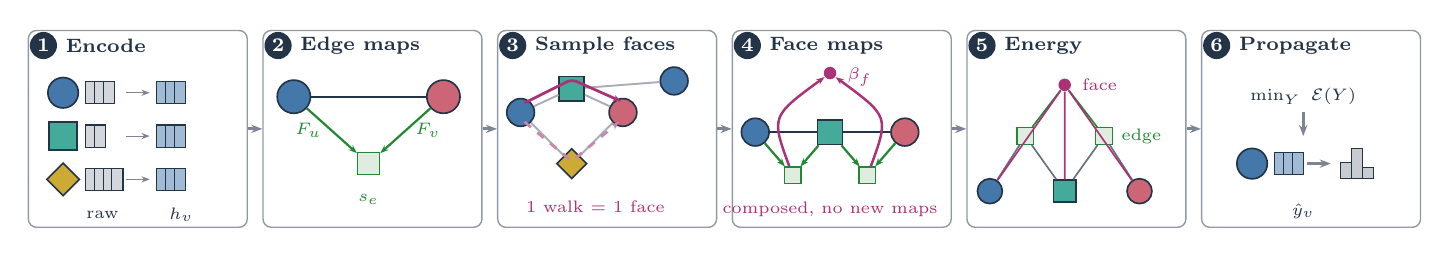
\begin{tikzpicture}
\def\W{2.98}
\foreach \i/\t in {0/Encode,1/Edge maps,2/Sample faces,3/Face maps,4/Energy,5/Propagate}{
  \node[stage] (B\i) at (\i*\W,0) {};
  \node[stnum] at ($(B\i.north west)+(0.2,-0.2)$) {\the\numexpr\i+1\relax};
  \node[sname] at ($(B\i.north west)+(0.36,-0.2)$) {\t};
}
\foreach \i in {0,...,4}{ \pgfmathtruncatemacro\j{\i+1} \draw[flow] (B\i.east)--(B\j.west); }
% 1 encode: typed raw features -> shared stalk space
\begin{scope}[shift={(0.3,-0.8)}]
 \foreach \y/\n/\w in {0/pap/3,-0.55/aut/2,-1.1/sub/4}{
   \ifx\n\relax\fi
 }
 \node[pap,fill=cA,minimum size=11pt] at (0.15,0) {};
 \node[aut,minimum size=10pt] at (0.15,-0.55) {};
 \node[sub,minimum size=12pt] at (0.15,-1.1) {};
 \foreach \y/\w in {0/3,-0.55/2,-1.1/4}{\foreach \k in {1,...,\w}{\node[vec=ink!20,minimum height=8pt] at (0.4+\k*0.11,\y) {};}
   \draw[-{Stealth[length=3pt]},ink!60] (0.95,\y)--(1.25,\y) node[midway,above=-2pt,small]{};
   \foreach \k in {1,...,3}{\node[vec=cA!50,minimum height=8pt] at (1.3+\k*0.11,\y) {};}}
 \node[small] at (0.65,-1.55) {raw};
 \node[small] at (1.65,-1.55) {$h_v$};
\end{scope}
% 2 restriction maps on one edge
\begin{scope}[shift={(\W+0.25,-0.85)}]
 \node[pap,fill=cA,minimum size=12pt] (u) at (0.15,0) {};
 \node[pap,fill=cB,minimum size=12pt] (v) at (2.05,0) {};
 \node[est,minimum size=8pt] (es) at (1.1,-0.85) {};
 \draw[ed] (u)--(v);
 \draw[mp] (u) -- node[small,left,text=grn]{$F_u$} (es);
 \draw[mp] (v) -- node[small,right,text=grn]{$F_v$} (es);
 \node[small,text=grn] at (1.1,-1.3) {$s_e$};
\end{scope}
% 3 sampling: walks
\begin{scope}[shift={(2*\W+0.3,-1.05)}]
 \node[pap,fill=cA,minimum size=10pt] (s1) at (0,0) {};
 \node[aut,minimum size=9pt] (s2) at (0.65,0.3) {};
 \node[pap,fill=cB,minimum size=10pt] (s3) at (1.3,0) {};
 \node[sub,minimum size=11pt] (s4) at (0.65,-0.65) {};
 \node[pap,fill=cA,minimum size=10pt] (s5) at (1.95,0.4) {};
 \draw[ed,ink!40] (s1)--(s2)--(s3) (s1)--(s4)--(s3) (s2)--(s5);
 \draw[-{Stealth[length=3pt]},rose,line width=1pt,rounded corners=2pt] ($(s1)+(0.05,0.12)$)--($(s2)+(0,0.12)$)--($(s3)+(-0.02,0.14)$);
 \draw[-{Stealth[length=3pt]},rose!60,line width=1pt,dashed] ($(s1)+(0.05,-0.12)$)--($(s4)+(0,0.03)$)--($(s3)+(-0.05,-0.12)$);
 \node[small,text=rose] at (0.95,-1.2) {1 walk = 1 face};
\end{scope}
% 4 face maps composed from edge maps
\begin{scope}[shift={(3*\W+0.3,-1.3)}]
 \node[pap,fill=cA,minimum size=10pt] (q1) at (0,0) {};
 \node[aut,minimum size=9pt] (q2) at (0.95,0) {};
 \node[pap,fill=cB,minimum size=10pt] (q3) at (1.9,0) {};
 \draw[ed] (q1)--(q2)--(q3);
 \node[est] (e1) at (0.475,-0.55) {};
 \node[est] (e2) at (1.425,-0.55) {};
 \draw[mp] (q1)--(e1); \draw[mp] (q2)--(e1); \draw[mp] (q2)--(e2); \draw[mp] (q3)--(e2);
 \node[fst] (zf) at (0.95,0.75) {};
 \draw[-{Stealth[length=3pt]},rose,line width=.9pt] (e1)..controls (0.2,0.2) .. (zf);
 \draw[-{Stealth[length=3pt]},rose,line width=.9pt] (e2)..controls (1.7,0.2) .. (zf);
 \node[small,anchor=west,text=rose] at (1.05,0.7) {$\beta_f$};
 \node[small,text=rose] at (0.95,-0.98) {composed, no new maps};
\end{scope}
% 5 energy on three levels
\begin{scope}[shift={(4*\W+0.3,-0.75)}]
 \node[fst] (z) at (0.95,0.05) {};
 \node[small,anchor=west,text=rose] at (1.05,0.05) {face};
 \node[est] (e0) at (0.45,-0.6) {};
 \node[est] (e1) at (1.45,-0.6) {};
 \node[small,anchor=west,text=grn] at (1.55,-0.6) {edge};
 \node[pap,fill=cA,minimum size=9pt] (n1) at (0,-1.3) {};
 \node[aut,minimum size=8pt] (n2) at (0.95,-1.3) {};
 \node[pap,fill=cB,minimum size=9pt] (n3) at (1.9,-1.3) {};
 \draw[grn,line width=.6pt] (z)--(e0) (z)--(e1);
 \draw[ink!70,line width=.6pt] (n1)--(e0) (n2)--(e0) (n2)--(e1) (n3)--(e1);
 \draw[rose,line width=.6pt] (z)--(n1) (z)--(n2) (z)--(n3);
\end{scope}
% 6 minimise & predict
\begin{scope}[shift={(5*\W+0.3,-0.85)}]
 \node[small] (en) at (1.0,0) {$\min_Y\ \mathcal{E}(Y)$};
 \draw[flow] (1.0,-0.2)--(1.0,-0.5);
 \node[pap,fill=cA,minimum size=11pt] (o) at (0.35,-0.85) {};
 \foreach \k in {1,...,3}{\node[vec=cA!50,minimum height=8pt] at (0.6+\k*0.11,-0.85) {};}
 \draw[flow] (1.05,-0.85)--(1.35,-0.85);
 \foreach \k/\h in {1/6,2/11,3/4}{\node[vec=ink!25,minimum height=\h pt,anchor=south] at (1.4+\k*0.14,-1.05) {};}
 \node[small] at (1.0,-1.45) {$\hat y_v$};
\end{scope}
\end{tikzpicture}
\end{document}
